% !TEX root = ./../main.tex
\chapter{Free energy calculations}
The preliminary results in \cite{ourPaper} and summarized in section~\ref{sec:NPMembraneInt} of the charged ligand translocation across the membrane are made using the standard \martini \ac{FF} with a cut--off method for treating the electrostatic interactions. Unfortunately, as we have seen in chapter~\ref{chap:EmpiricalFF}, such method poorly describe the processes that involve the electrostatic interaction and hence it underestimates the energy barriers of the processes between ions, water molecules and hydrophobic molecules. Moreover the use of the standard \martini water model does not improve the energy barriers estimation.

The pathway to improve the model is the use of the \ac{PME} method to better describe the electrostatic interaction and the use of the \ac{PW} model to improve the behavior of the water solvent at a \ac{CG} level. For a comparison to be made, the idea, is to follow the procedure describe in section~\ref{sec:preliminaryMetadyn} and, with metadynamics runs, try to estimate the energy barrier of the anchoring process with the use of the \ac{PME} alone and in combination with the \ac{PW} model. 

Preliminary, some tests about the use of the \ac{PME} method and the \ac{PW} model with a pure \ac{POPC} bilayer was performed. Then metadynamics runs for obtaining the \ac{FES} of the anchoring process involving both the striped (\ac{MUS}:\ac{OT} $1$:$1$) and the random (\ac{MUS}:\ac{OT} $1$:$1$) \acp{NP} were performed with the use of the \ac{PME} alone and in combination with the \ac{PW}. 
%In view of the results, then, as better described in the next chapter, unbiased \ac{MD} runs with the use of \ac{PME} and \ac{PW} involving all the \ac{NP} configurations were performed in order to investigate a possible change in the kinematic of the all the \ac{NP}--membrane interaction process.

\section{Metadynamics: system set--up and issues}
%tentativi di convergenza con bound
The idea for a comparison to be made on the basis of free energy calculations is to obtain the \ac{FES} of the anchoring process of one charged ligand as described in section~\ref{sec:preliminaryMetadyn} using the different \ac{NP} configurations with the new \martini models. In order to understand if this more sophisticated \ac{CG} models is suitable to better describe such process, a comparison with an atomistic simulation\footnote{All \acs{MD} simulations and metadynamics runs with the atomistic \ac{FF} are performed by Federica Simonelli in her PhD study.} is necessary. In this way we can investigate if a more realist description can be obtained with a \ac{CG} model in order to use it for future applications.

To summarize briefly, the process that I will consider for the \ac{FES} estimation of the ligand anchoring is composed of two steps: the first, called forward process: from the hydrophobic state to one anchor state; the second, backward process: from the anchored state to the hydrophobic state again. 

\paragraph{\textbf{system set--up}} In all of my \ac{MD} runs the membrane bilayer is made of $256$ \ac{POPC} lipids per leaflet. I will consider both the striped (\ac{MUS}:\ac{OT} $1$:$1$) and the random (\ac{MUS}:\ac{OT} $1$:$1$) \acp{NP}. The simulation box is neutralized with $30$ counteracting Na$^+$ ions\footnote{The \martini model for ions, especially for Na$^+$ and Cl$^-$, associates the ion plus the hydration shell to a bead of type Qd positively charged and Qa negatively charged, respectively.} and filled by water. In figure~(\ref{fig:startFrameEx}) is shown an example of the starting configuration for a striped (\ac{MUS}:\ac{OT} $1$:$1$) \ac{NP} in the hydrophobic state. The charged ligand for the anchoring process is choses so as to be the lowest ligand attached to the \ac{NP} core. The initial configuration frames with the \ac{PW} are obtained from the initial configuration frames with the standard \martini water using a python script that convert the standard \martini water to the \ac{PW} bead. With the \ac{PW} an equilibration run with the parameters shown in the third column of table~(\ref{tab:inputParam}) is necessary to correctly stabilize the system. For what concern the metadynamics input parameters, if not differently specified, they are summarized in table~(\ref{tab:metadynParam}).
\begin{SCfigure}[][!ht]
	\centering
	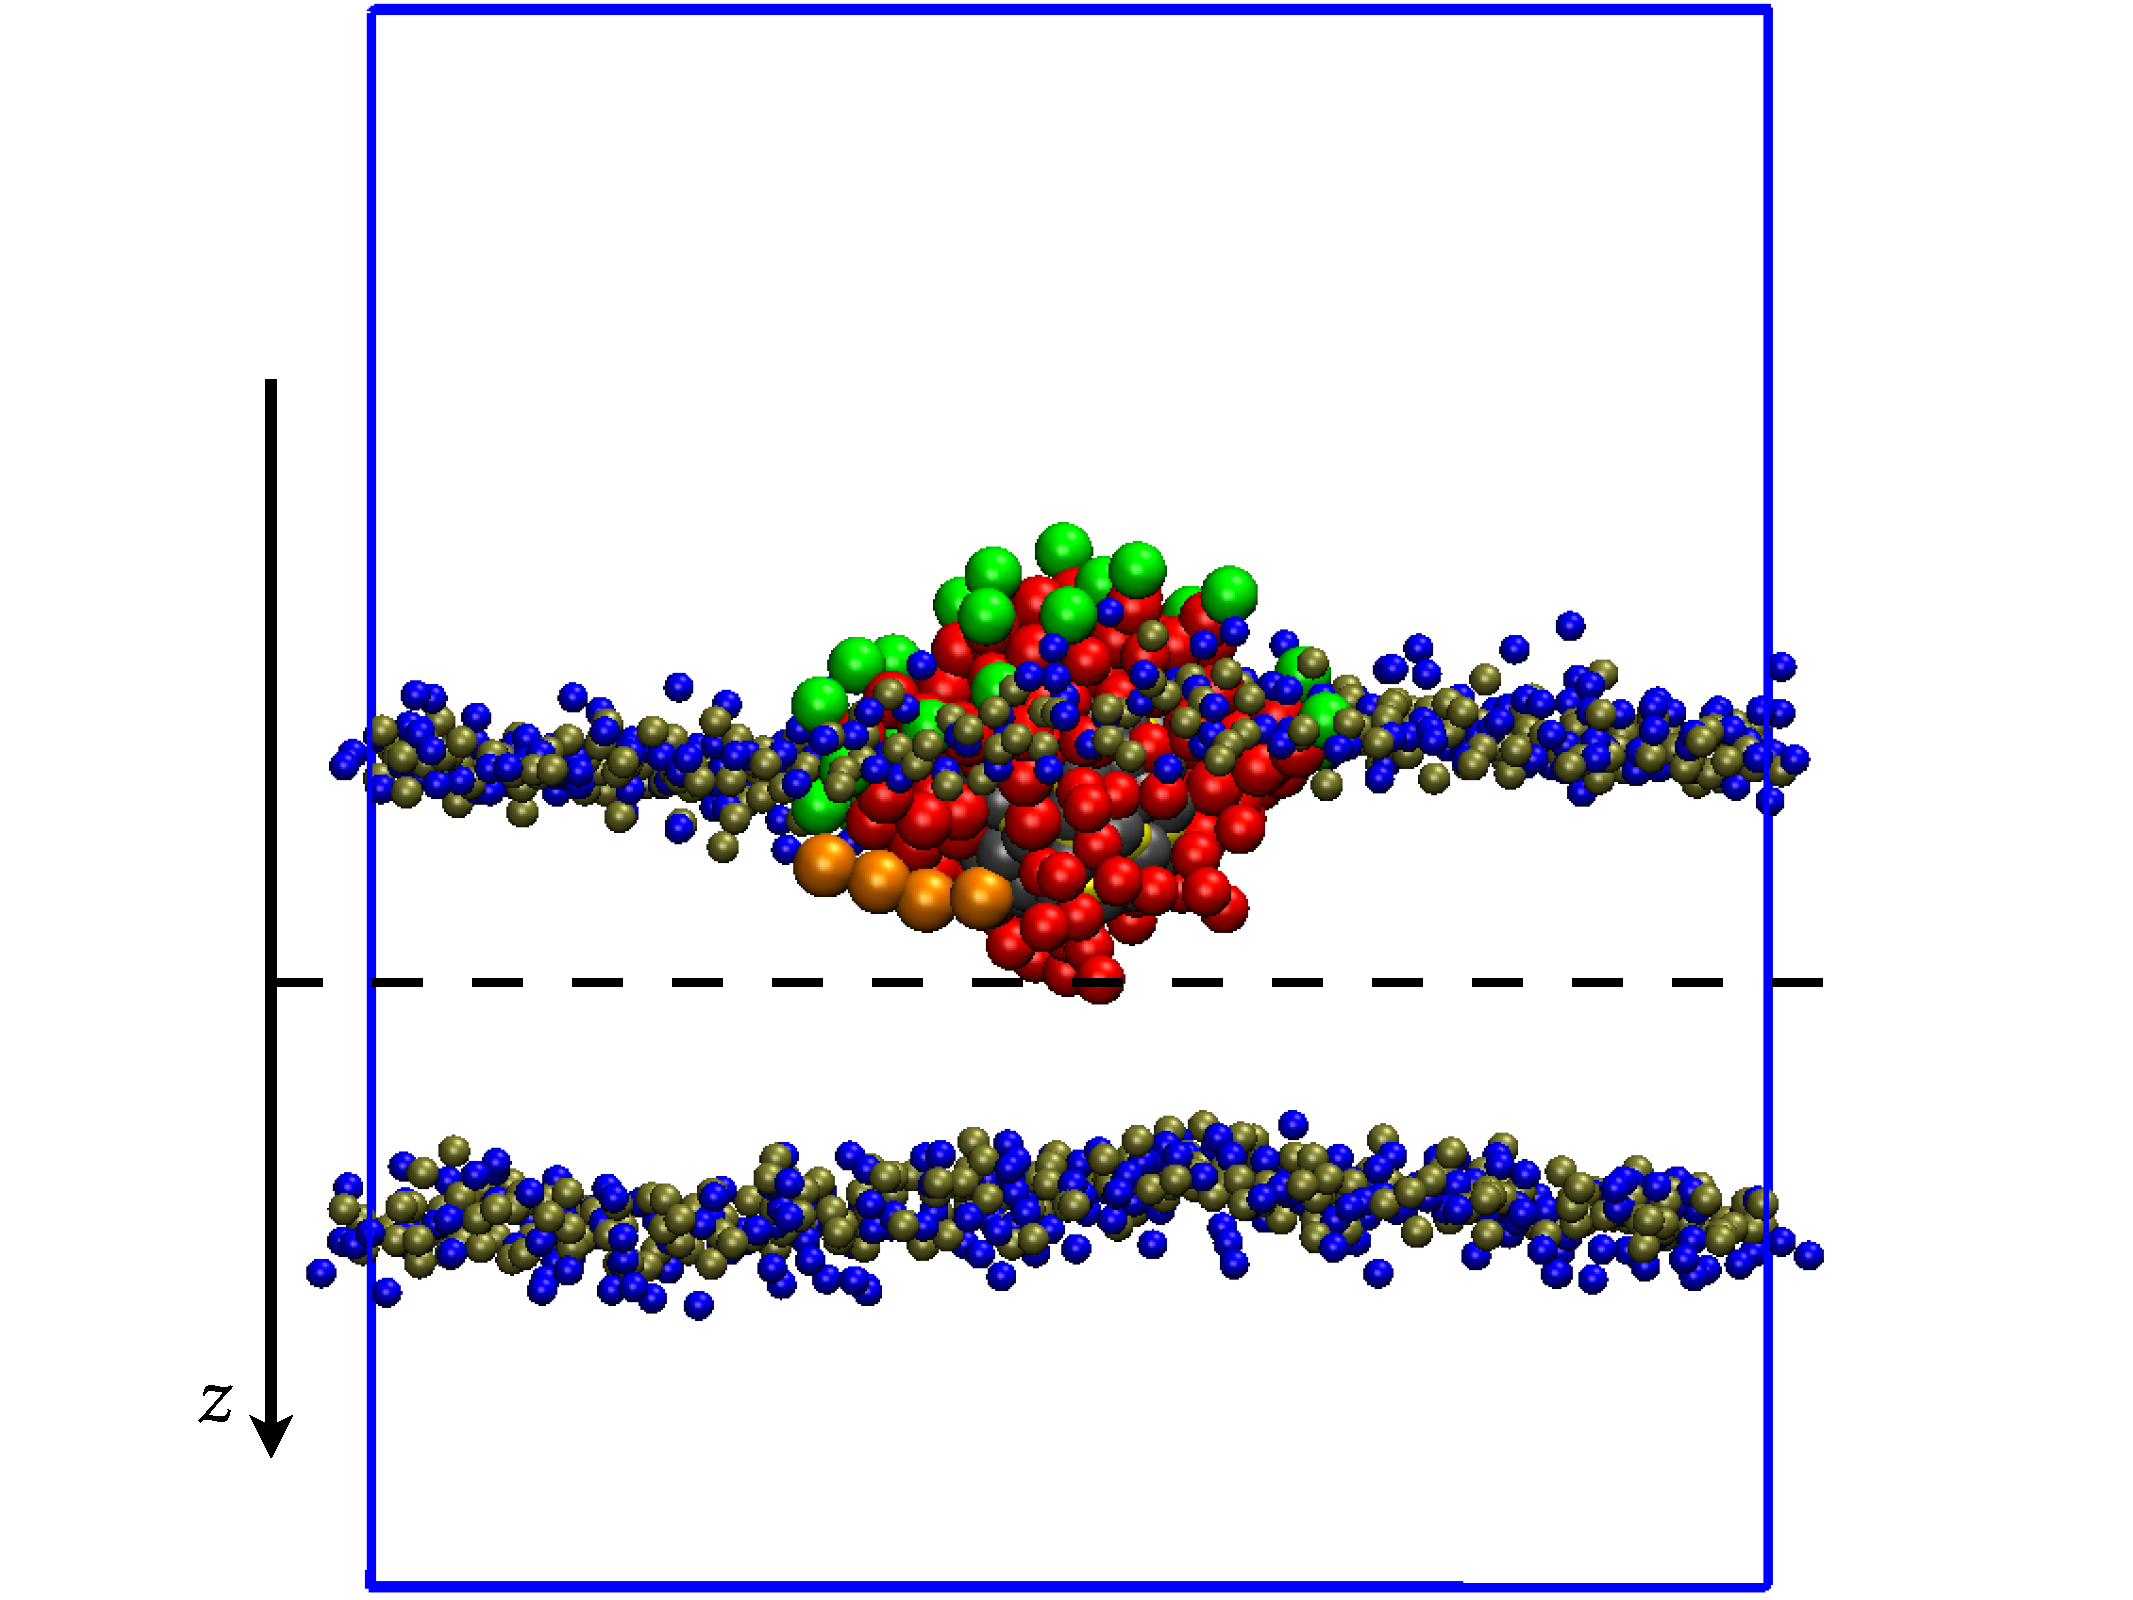
\includegraphics[width=0.5\textwidth]{./img/patchedHydrophobic}
	\caption{Example of a starting configuration of a metadynamics run of a striped (\ac{MUS}:\ac{OT} $1$:$1$) \ac{NP} in the hydrophobic state. Color code as in figure~(\ref{fig:threeProcess}). The charged ligand chosen for the anchoring process is in pink. The blue contour is the simulation box. Water beads and lipid tails are not shown.}
	\label{fig:startFrameEx}
\end{SCfigure}

\paragraph{\textbf{CV issues}} The \ac{CV} chosen to describe the anchoring process is the $z$ component of the distance between the center of the charged bead and the \ac{COM} of the bilayer. Although this \ac{CV} is a very intuitive and simple, with the introduction of the \ac{PME} method, and more accentuated with the \ac{PW} model, we found that it suffers of some issues. When I perform the metadynamics runs with the \ac{PME} and \ac{PW}, in accordance with the atomistic results, it is observed that the anchored state is more stable than with the standard \martini models: the increase of the model accuracy make the interaction between the negatively charged bead and the positively charged choline group of the lipid heads of the opposite leaflet, stronger than with the standard \martini. The same apply with the \ac{PW} beads. Hence, like in figure~(\ref{fig:engulfment}), we observe that when the metadynamics try to dis--anchor the charged bead in the backward process, it pull back the lipid heads slightly deforming the opposite leaflet of the bilayer. This results in a worse estimation of the \ac{CV} because the charged ligand is in the hydrophobic region near the entrance leaflet but still in contact with one or two lipid heads of the opposite leaflet.
\begin{SCfigure}[][h!t]
	\centering
	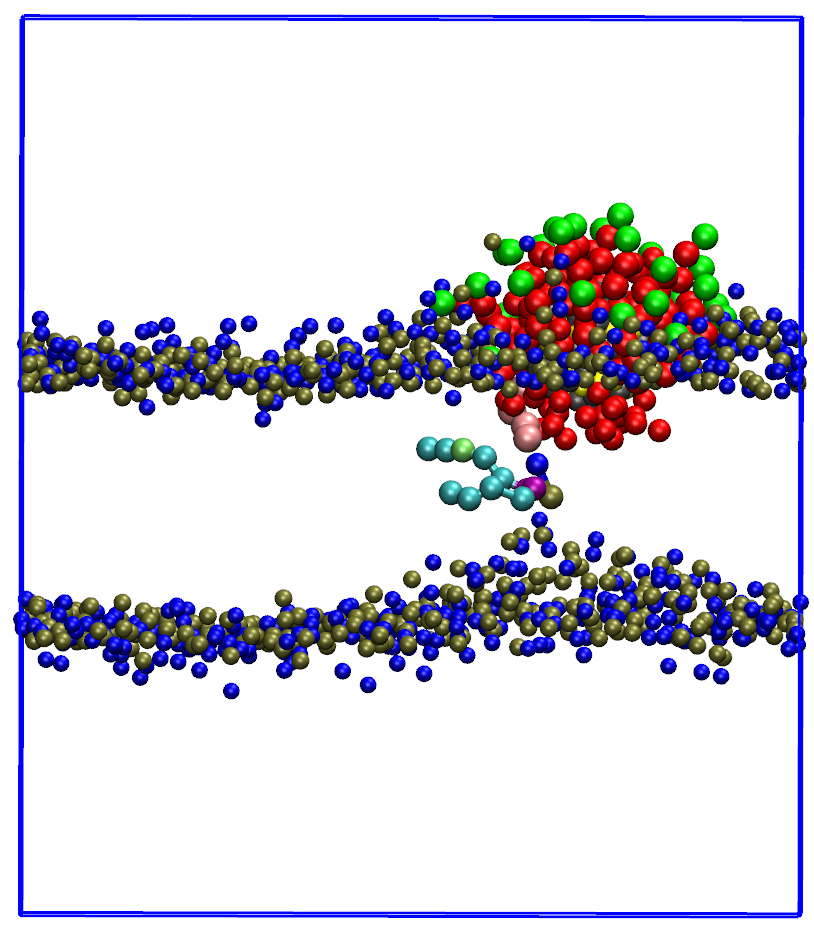
\includegraphics[width=0.5\textwidth]{./img/patchedEngulfment}
	\caption{Detail of the engulfment effect in the anchoring leaflet when the ligand tends to dis--anchor. Color code as in figure~(\ref{fig:threeProcess}). Lipid tails are shown in cyan while the glycerol group is represented by the violet beads. Water and other lipid tails are not shown. The choline group (blue bead) is in contact with the charged bead of the ligand (pink beads) and the lipid tails are horizontal instead of vertical as they usually are.}
	\label{fig:engulfment}
\end{SCfigure}
Another import issue as the simulation time increase and related to the previous issues, is the loss of the ability by the \ac{CV} to well distinguish the two states, although the convergence has not yet reached. In figure~(\ref{fig:NPDist}) the red line is the \ac{CV}. In the region $z > 1$ the ligand have crossed the \ac{COM} of the bilayer and it is anchored in the opposite leaflet. For $z < -1$ the ligand is near the \ac{NP}'s leaflet in the hydrophobic state. While for $-1 < z < 1$ the ligand is in the hydrophobic region of the membrane but it may be in contact with the lipid head beads of the opposite leaflet. Hence inside the dashed black lines there is a region of the \ac{CV} space in which the two states are overlapping. This issue leads in a underestimation of the forward wall of the one anchor \ac{FES} because it tend to lower the saddle point while the metadynamics is still sampling the anchored state.
\begin{figure}[!ht]
	\centering
	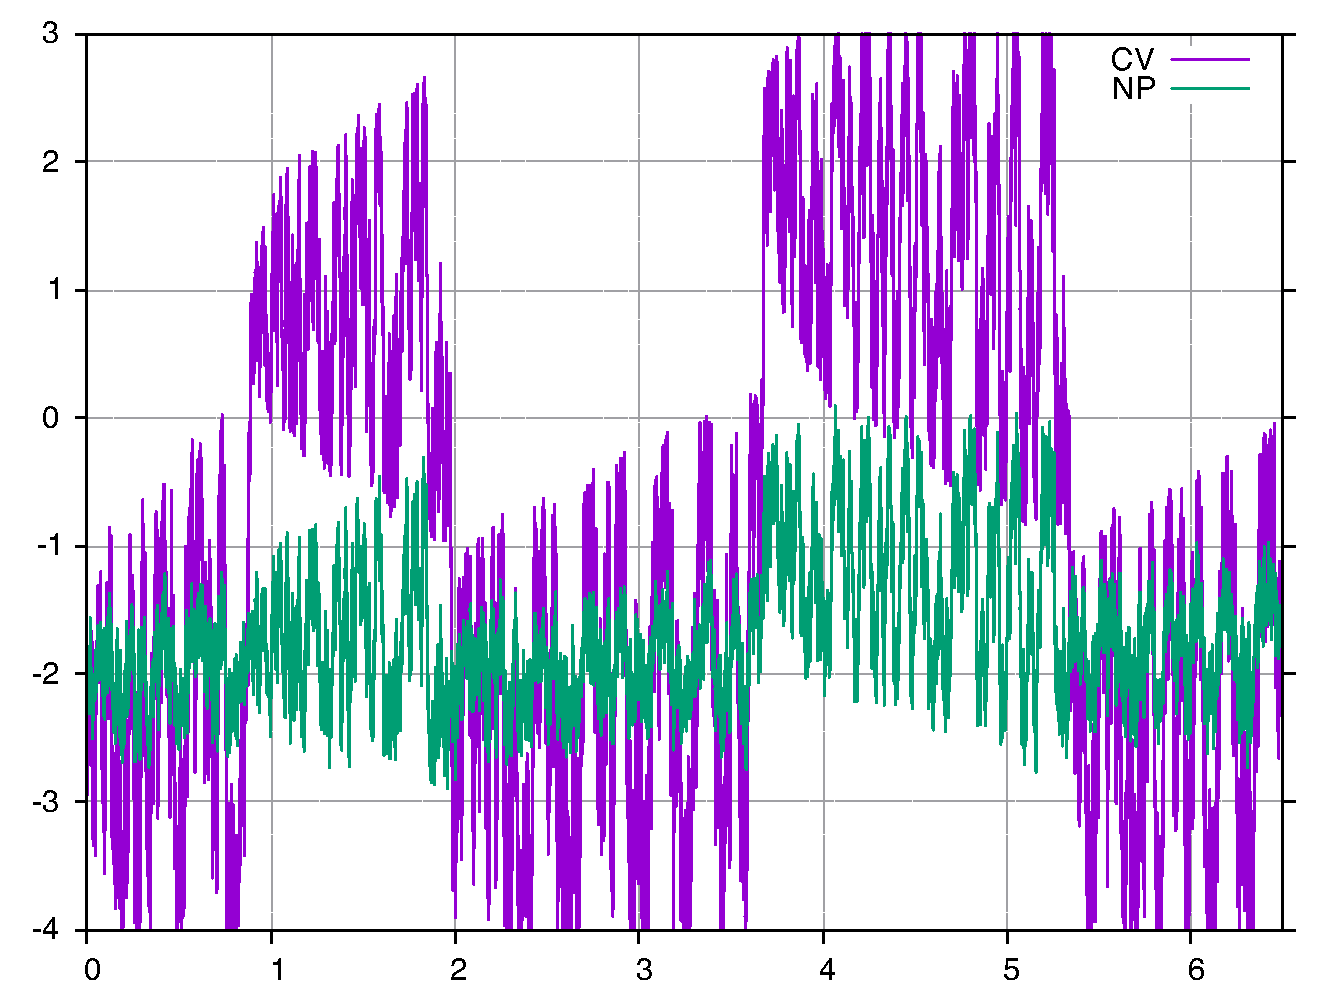
\includegraphics[width=0.7\textwidth]{./img/results/NPDistance/NPDist}
	\caption{Correlation between the \acs{CV} (red) and the $z$ component of the distance between the \acs{COM} of the \acs{NP} and the \acs{COM} of the bilayer (green) as a function of the simulation time. The region of the \acs{CV} space inside the dashed black lines is the overlapping region. Data obtained from a $6.5$~$\mu$s metadynamics run of a striped (\acs{MUS}:\acs{OT} $1$:$1$) \acs{NP} with \acs{PW}.}
	\label{fig:NPDist}
\end{figure}

%Moreover, since the interaction with the lipid heads is stronger, 

\paragraph{\textbf{convergence problems}} An important issue related to this process is the achievement of the convergence, essential in the \ac{FES} estimation. Our metadynamics runs have not reached the convergence, even in tens of microseconds of simulation, as we can see from figure~(\ref{fig:NPDist}) (red) of a $6.5$~$\mu$s test run in which we try to reach the convergence\footnote{In this run in an attempt to speed up the achievement of the convergence, in addition to the metadynamics bias, I use two other harmonic bias to limit the sampled region. Un upper bias which is activated when the charged bead is far from the bilayer \acs{COM} for more than $3$~nm and a lower bias when the charged bead is far from the bilayer \acs{COM} for more than $-4$~nm. The elastic constant is chosen $k = 100$~kJ/mol for both.}. This is prevalently due to the just described issues associated to the \ac{CV}. But also, in accordance with my unbiased simulations and the atomistic results, because the energy barriers associated to the two metastable state are much higher than what are estimated in \cite{ourPaper}, slowing down the reaching of the convergence. Another issues is related to stronger interaction between the charged bead and the \ac{PW} beads and the charged bead and the lipid heads. From the metadynamics runs, for the random and more pronounced for the striped \acp{NP}, we observe that, respect to the standard \martini model, the charged ligand spend a not negligible time completely soaked in the water phase ($z>-2$). This leads to sample a region of the \ac{CV} space useless for one anchor \ac{FES} estimation and tend to slow down the achievement of the convergence. Another undesired process that we observe as the simulation time increase, is a small drag of the \ac{NP} inside the bilayer by the charged ligand in the anchored state. From figure~(\ref{fig:NPDist}), since the stronger interaction with water, we see that when the charged bead is approaching the water phase of the opposite leaflet ($z>2$) it is not only due to the ligand itself but also because the \ac{COM} of the \ac{NP} tend to approach the \ac{COM} of the bilayer (green). Despite this can be an important molecular process in order for a comparison to be made, we must not sample the phase phase associated to the movement of the \ac{COM} of the \ac{NP} since we are interested in the \ac{FES} associated to the anchoring process only.

\paragraph{\textbf{worse estimation of the FES}} From the previous explanations it is clear that following the procedure outlined in \cite{ourPaper} leads to a worse estimation of the \ac{FES} associated to the anchoring process. In particular all these issues suggest a different pathway, at molecular level, for the forward process respect to the backward process and that some other \acp{CV} are missing. Hence, using the same \ac{CV}, instead to try to estimate the whole \ac{FES}, we can try to estimate the energy wall associated to the forward process and, separately, the energy wall associated to the backward process. For the estimation of the energy wall of the forward process we need to start the metadynamics runs in the hydrophobic state and stop it when the ligand reach the anchored state. For the backward process we need to do the contrary: start the metadynamics from the anchored state and stop it when the ligand return to \ac{NP} leaflet. Then we can compare the new results with the standard \martini model and the atomistic one.
%la usiamo per stimare la barriera di andata e ritorno

\section{Forward process}
I have performed ten metadynamics runs starting at hydrophobic state for each of the following ``configurations'': striped (\ac{MUS}:\ac{OT} $1$:$1$) with \ac{PME}; striped (\ac{MUS}:\ac{OT} $1$:$1$) with \ac{PME} and \ac{PW}; random (\ac{MUS}:\ac{OT} $1$:$1$) with \ac{PME} and \ac{PW}. This runs are suitable for the estimation of the forward energy wall.

For a comparison between different models to be made all the distance variables involving the bilayer (e.g. the chosen \ac{CV}) are scaled by the ratio between the thickness of a pure \ac{POPC} bilayer with the atomistic \ac{FF} and the one obtained with the \ac{CG} \ac{FF}. This ratio is calculated from the bilayer's thickness shown in table~(\ref{tab:POPCData}).
 
\subsection{Models comparison}
%striped models comparison (Standard, PME, PME & PW, Atomistico)
A comparison of the forward wall obtained for the striped (\ac{MUS}:\ac{OT} $1$:$1$) \ac{NP} with different models is shown in figure~(\ref{fig:forwardWall}) and in table~(\ref{tab:hydroTime}) are summarized the average height of the barrier with the \ac{CG} models; the height of the barrier in the atomistic case is, instead, $\Delta G = 134 \pm 5$~kJ/mol. For the \ac{PME} and the \ac{PME}+\ac{PW} versions is shown an average over ten simulations each. For the STD version is shown an average over eight simulations. The atomistic version is obtained over an average of two simulations. The error is estimated using the standard error as in the procedure described in section~\ref{sec:metadynamics}. As we can see, increasing the accuracy of the \ac{CG} model, in particular with the use of the \ac{PW} model, the \ac{CG} results are approaching the atomistic one. Despite the shift of the \ac{CV} respect to the thickness of a pure \ac{POPC} bilayer with the atomistic and the \ac{CG} models, we see that the minimum is not well align. This can be because in the metadynamics runs the thickness of the bilayer in the \ac{CG} models may change: for example, with the \ac{PW} and a striped \ac{NP} the thickness is in the range of $4$~nm to $4.4$~nm. The same slightly apply in the atomistic case too.

As we shall see later, the order of magnitude of the energy barrier is consistence with my unbiased simulations of all \acp{NP} with the \ac{PW} in which for ten of microseconds no anchor process is observed. This suggest that the energy wall is much higher than what is observed in \cite{ourPaper}. Another sign of the increasing of the energy wall as the \ac{CG} model accuracy increase, is the time spent by the \ac{NP} in the hydrophobic state. In table~(\ref{tab:hydroTime}) is shown a comparison of the average time spent by the \ac{NP} in the hydrophobic state between different \ac{CG} models.
\begin{table}[h!t]
	\centering
	\begin{tabular}{lcccc}
		\toprule
		\,					& STD$^a$	& \acs{PME}$^b$	& \acs{PME}$+$\acs{PW}$^b$  \\ \toprule
	$\overline{t_{h}}$ [ns]	& $\sim 140$& $\sim 215$	& $\sim 982$			 	\\ \midrule
	$\Delta G$ [kJ/mol] 	& $26 \pm 2$& $36 \pm 4$	& $100 \pm 5$				\\ \bottomrule
	\end{tabular}
	\caption{Summary of the metadynamics results of the striped (\acs{MUS}:\acs{OT} $1$:$1$) \acs{NP}. $\overline{t_h}$ is the average time spent in the hydrophobic state. $\Delta G$ is the average height of the forward energy wall; the error is the error standard. \footnotesize $^a$ Data obtained from \cite{ourPaper}. $^b$ Data obtained from my \acs{MD} runs.}
	\label{tab:hydroTime}
\end{table}

\begin{figure}[pth]
	\centering
	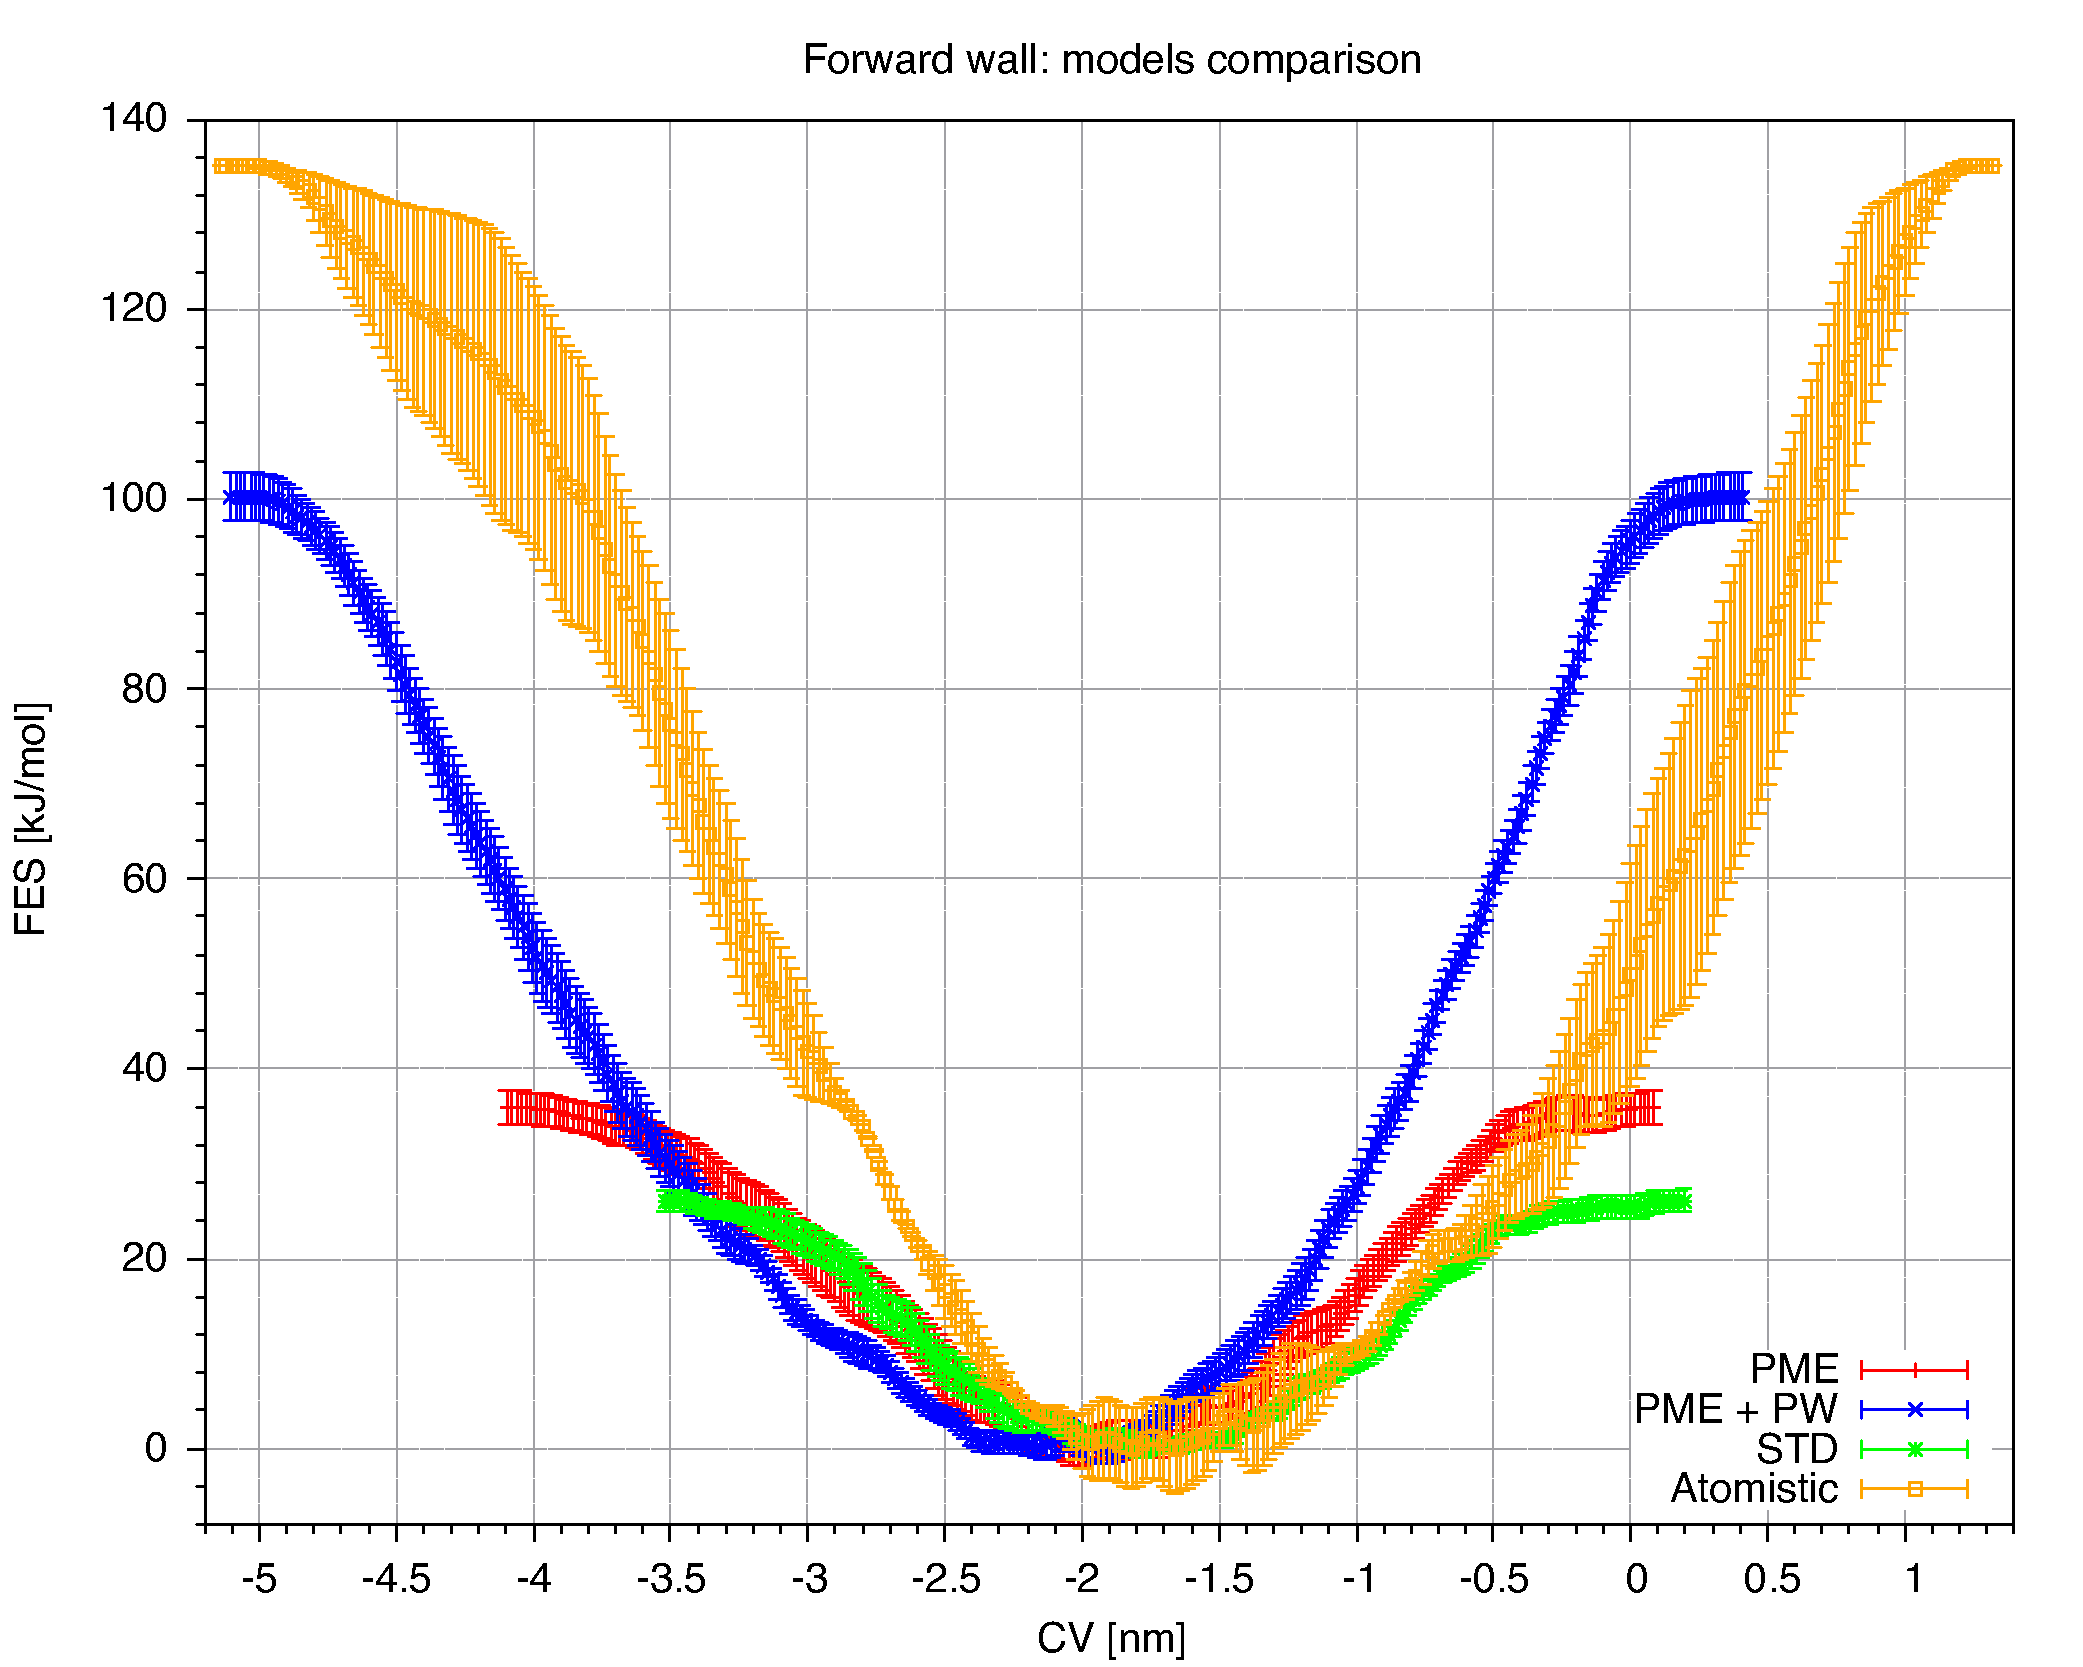
\includegraphics[width=0.7\textwidth]{./img/results/FESModelComparison/forwardWall}%
	\caption{\acs{FES} of the forward energy wall in function of the \acs{CV} in a comparison with different models.}%
	\label{fig:forwardWall}%
	\vspace*{\floatsep}%
	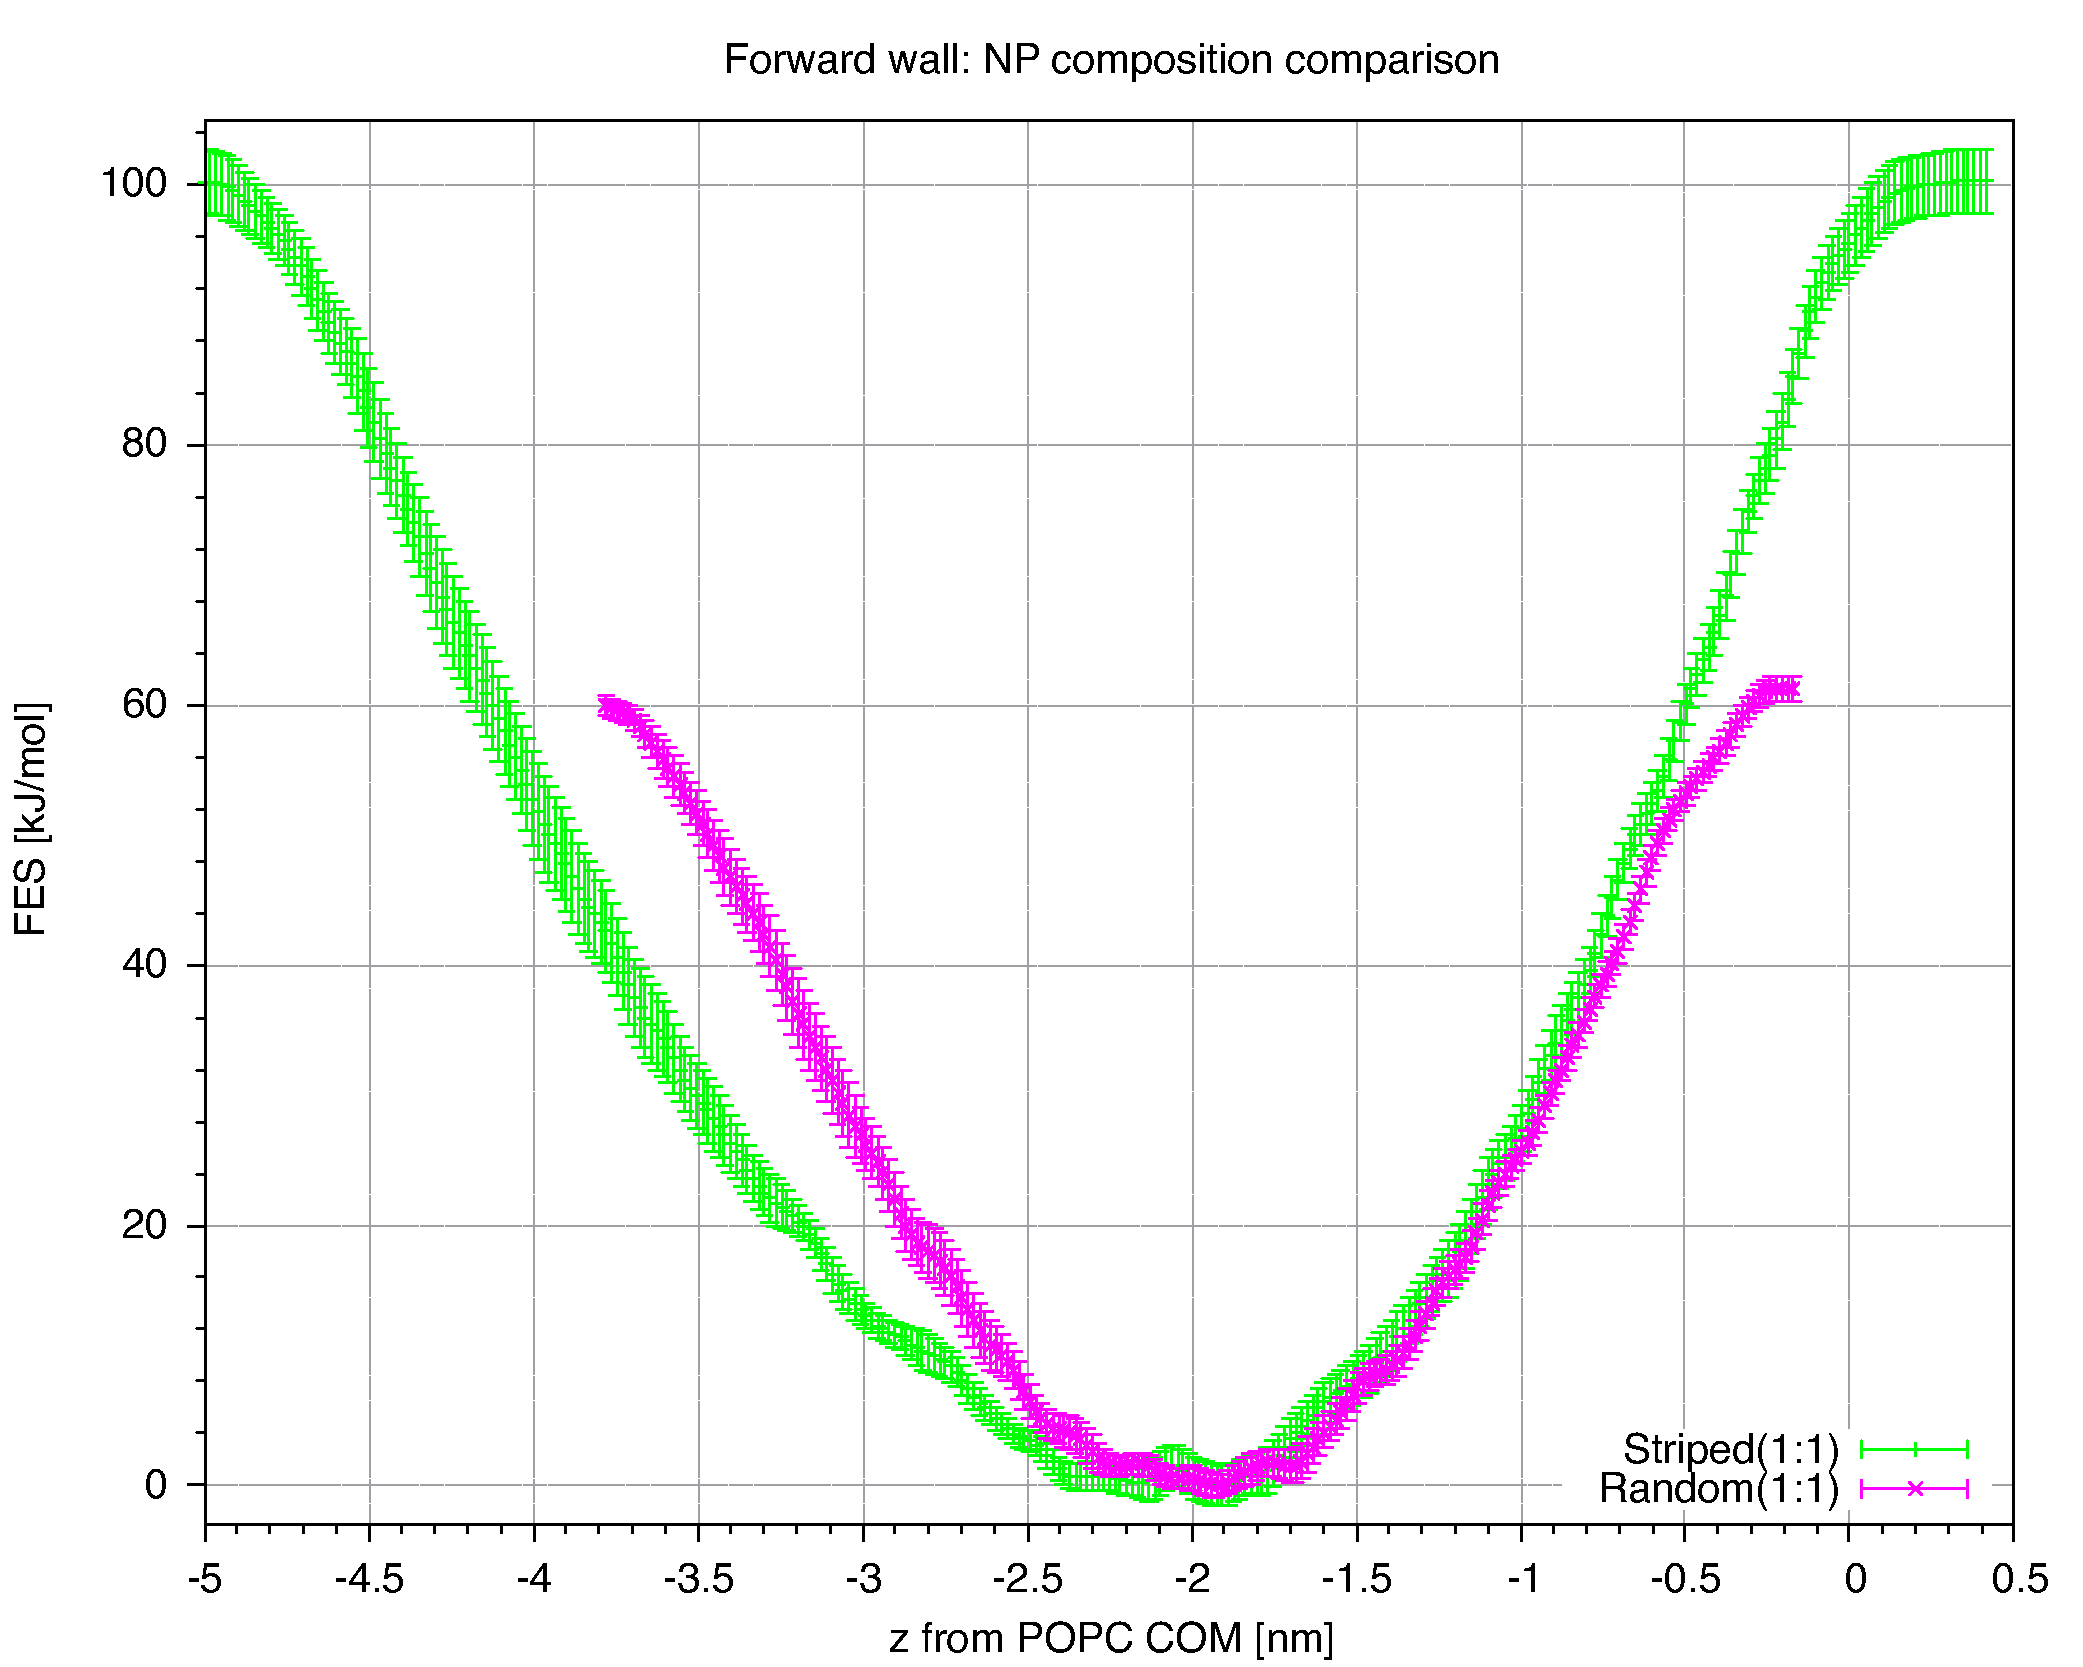
\includegraphics[width=0.7\textwidth]{./img/results/FESModelComparison/forwardWallRP}%
	\caption{\acs{FES} of the forward energy wall in function of the \acs{CV}. The green is for the striped \acs{NP}. The magenta is for the random one.}%
	\label{fig:forwardWallRP}
\end{figure}

\subsection{Striped and random comparison}
%metadinamiche patched e random con PME e PW
The metadynamics runs performed allow us for a comparison of the forward energy wall for both striped (\ac{MUS}:\ac{OT} $1$:$1$) and random (\ac{MUS}:\ac{OT} $1$:$1$) \acp{NP} with the \ac{PW}. The comparison is shown in figure~(\ref{fig:forwardWallRP}) and in table~(\ref{tab:hydroTimeRP}). We can confirm the trend observed in \cite{ourPaper}: the striped (\ac{MUS}:\ac{OT} $1$:$1$) \ac{NP} has an higher energy wall for the hydrophobic to one anchor state transition than that for the random (\ac{MUS}:\ac{OT} $1$:$1$) \ac{NP}. Moreover in table~(\ref{tab:hydroTimeRP}) is show a comparison of the average time spent by the \ac{NP} in the hydrophobic state between the striped and the random configuration.
\begin{table}[h!t]
	\centering
	\begin{tabular}{lcccc}
		\toprule
		\,					& striped		& random		\\ \toprule
	$\overline{t_{h}}$ [ns]	& $\sim 982$	& $\sim 413$	\\ \midrule
	$\Delta G$ [kJ/mol] 	& $100 \pm 5$ 	& $61 \pm 2$	\\ \bottomrule
	\end{tabular}
	\caption{Comparison of the metadynamics result with the \ac{PW} model for the striped and random \acp{NP}. $\overline{t_h}$ is average time spent by the \acs{NP} in the hydrophobic state. $\Delta G$ is the average height of the forward energy wall; the error is the error standard. Data obtained from my \acs{MD} runs.}
	\label{tab:hydroTimeRP}
\end{table}

 
\section{Backward process: preliminary results}


\section{Discussion of the results}
In order to understand the order of magnitude of the forward energy wall, the process of the charged bead translocation through the membrane can be thermodynamically compared to two main processes: the ion membrane translocation and the lipid flip--flopping in a pure \ac{POPC} bilayer.

For the first comparison, in \cite{PW} the authors have computed the \ac{FES} of the translocation of one Na$^+$ and one Cl$^-$ ions across a \acs{DPPC} membrane using umbrella sampling and the \ac{WHAM} with the standard \martini \ac{FF}, with the \ac{PW} alone and with \ac{PW}$+$\ac{PME}. The height of the barriers are summarized in table~(\ref{tab:ionTranslocation}). The same \ac{FES} for a \acs{DMPC} membrane was calculated by Khavrutskii \etal\, \cite{atomisticTranslocation} with an atomistic \ac{FF}. Since the \martini model for the \acs{DPPC} lipid also model the \acs{DMPC} lipid a comparison can be made and it is shown in table~(\ref{tab:ionTranslocation}). As one can see, from left to right, increasing the loyalty of the treatment of the electrostatic interaction the \martini \ac{FF} approach the results of the atomistic \ac{FF}, as we see also in figure~(\ref{fig:forwardWall}). Moreover for what concern the \ac{PW}$+$\ac{PME} result it are comparable to one obtained in our forward energy wall as we can see from table~(\ref{tab:hydroTimeRP}). Moreover in \cite{PW}, in accordance with the atomistic results in \cite{atomisticTranslocation}, for small cross membrane ions imbalance and only with the use of the \ac{PW} model and the \ac{PME} method, they observe some ion leakage without pore formation but still mediated by a water defect inside the membrane, called \textit{water finger} that help the ions to cross the hydrophobic region of the membrane.
%We remark that, these kind of phenomena, are totally absent using the standard \martini \ac{FF}. Hence, as already outlined, the importance to use a better treatment of the electrostatic interaction and a better model for water solvent.
\begin{table}[h!t]
	\centering
	\begin{tabular}{lcccc}
		\toprule	
		\,		& STD 	& \acs{PW} 	& \acs{PW}$+$\acs{PME} 	& atomistic	\\ \toprule
		Na$^+$	& $68.0$& $67.6$	& $78.6$				& $91.7$ 	\\ \midrule
		Cl$^-$	& $69.2$& $70.4$	& $99.0$				& $98.8$	\\ \bottomrule
	\end{tabular}
	\caption{Height of the energy barrier (in kJ/mol) for Na$^+$ and Cl$^-$ ion translocation across a bilayer. The \martini results are based on a \acs{DPPC} membrane and are taken from \cite{PW}. The atomistic are based on a \acs{DMPC} membrane and are taken from \cite{atomisticTranslocation}.}
	\label{tab:ionTranslocation}
\end{table}

For the second comparison, we refer to the work of Sapay \etal\, in \cite{Sapay2009}, in which the authors have calculated, using an atomistic \ac{FF} and through umbrella sampling, the \acp{FES} of a flip--flipping process of a lipid in several pure bilayers with different lipid composition, including a pure \ac{POPC} membrane. They pull a lipid head inside the hydrophobic core via a bias potential and found that the energy barrier of a lipid flip--flop in a \ac{POPC} membrane is of the order of $\sim 90$~kJ/mol. Moreover they observe that the flip--flopping process occur without a water pore formation, as in our case: the  ligand translocation occur without a pore formation. In principle this kind of comparison is more realistic than the previous one. This because the charged ligand has an hydrophobic chain, like a lipid, and because, instead of the ions case in which they start in the water phase, our ligand start near the lipid heads region of the entrance leaflet and in most cases the hydrophobic beads are already in contact with the hydrophobic region of the membrane. Despite this, our atomistic result give an energy barrier that is about $35$~kJ/mol greatest than the previous processes.















